
\chapter{Mathematical Definitions}

We are interested in constructing parametric polytopes for
mathematical exploration. An informal geometric
picture of a polytope has already been developed.
In this chapter we will develop a mathematical perspective of our problem
such that we can focus clearly on the computational aspects in the following
sections. 


\section{Vector Spaces}

Given a field (in the algebraic sense) of numbers, a vector of dimensionality
N is formed by an N-tuple of numbers in the field. A vector space must
be closed under element-wise addition with another vector and element-wise
multiplication by a scalar value. Symbolically, given $s \in F$ where $F$ is a
field, and $X,Y \in V$ where V is the vector space over $F$ then
$X+Y \in V$ and $s*x \in V$ implies our closure property.
In this paper we will primarily use
the real numbers in euclidean $N$ dimensional space, denoted as $\mathbb{R}^N$.
The term ``point" will generally be used to describe a vector that may
described using numerical values.

\section{Polytopes}

To quote H.S.M. Coxeter, ``A polytope is a geometrical figure bounded by portions of
lines, planes, or hyperplanes". We have already introduced the notion that a
polytope generalizes the notions of polygons and polyhedra, objects
that have been studied since antiquity. If we interpret a polytope in
one dimension, we may say that it is a line segment. Based on our previous
geometric intuition of these objects we may see that a polygon is constructed
from line segments and a polyhedron constructed from polygons. It is common
a common occurrence in geometrical definitions that a construct of dimensionality
$N$ will use objects of dimensionality $N-1$. We will formally define a polygon
and polyhedron now.

\subsection{Polygons}

A polygon is a circuit of line segments formed by points. Let us define our
number of points, N, as $V_1, V_2, ... V_N$. We will call these points
``vertices", and form the line segments between vertices by
$V_1 V_2, V_2 V_3, ... V_N V_1$
and call these ``edges". For our purposes we will only consider vertices existing
in the same plane, however this is not strictly necessary. The planer and
non-planar forms are called ``planar" and ``skew" respectively by Coxeter
\cite{Coxeter}.
A polygon forms an interior region and exterior region. The interior region
is finite, and is bounded by the edges of the polygon.

\subsection{Polyhedra}

A polyhedron will be defined by a finite set of polygons. Given polygons
$F_1, F_2, ..., F_N$ a polyhedron is a finite region bounded by these polygons.
These polygons are called faces of the polyhedron. 


\section{Combinatorial Representation of a Polytope}

Our initial intuition and definitions of polytopes are far from concrete enough to
implement in a computational environment. In this section we will define a
polytope using simplices, which are more constrained and allow us to
more easily infer properties of the polytopes.

\subsection{Simplices}

A simplex (plural simplices) in N dimensional space is the minimal set of
points whose convex hull form a closed subset in a space of dimensionality N.
In set notation, for $M$ linearly independent points ($P$) a simplex is the
linear combination of these points.
\begin{equation}
\{\sum_{n=1}^{M}s_n*P_n | \sum_{n=1}^{M} s_n = 1\}
\end{equation}

It is often thought
of as the generalization of a tetrahedra into N dimensions. In one dimensional
space, this is a closed interval or line segment. In two dimensions it is the
triangle, and in three it is the tetrahedra. These are called a 1-simplex,
2-simplex, and 3-simplex respectively. Figure \ref{fig:simplices} shows
some examples of the connectivity between vertices in simplices.


\begin{figure}[h!]
  \centering
    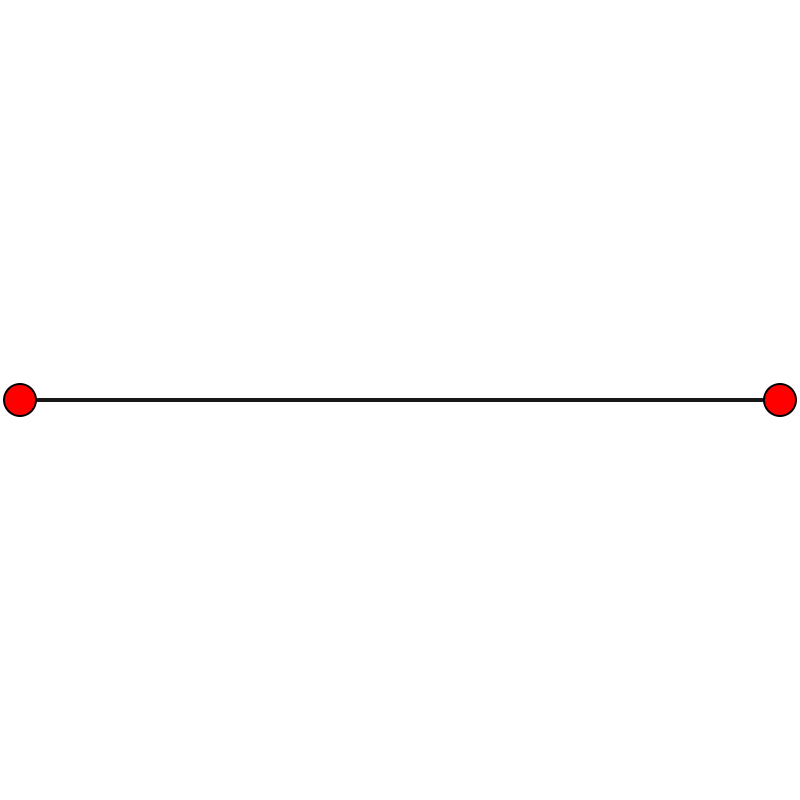
\includegraphics[width=0.4\textwidth]{img/800px-1-simplex_t0.png}
    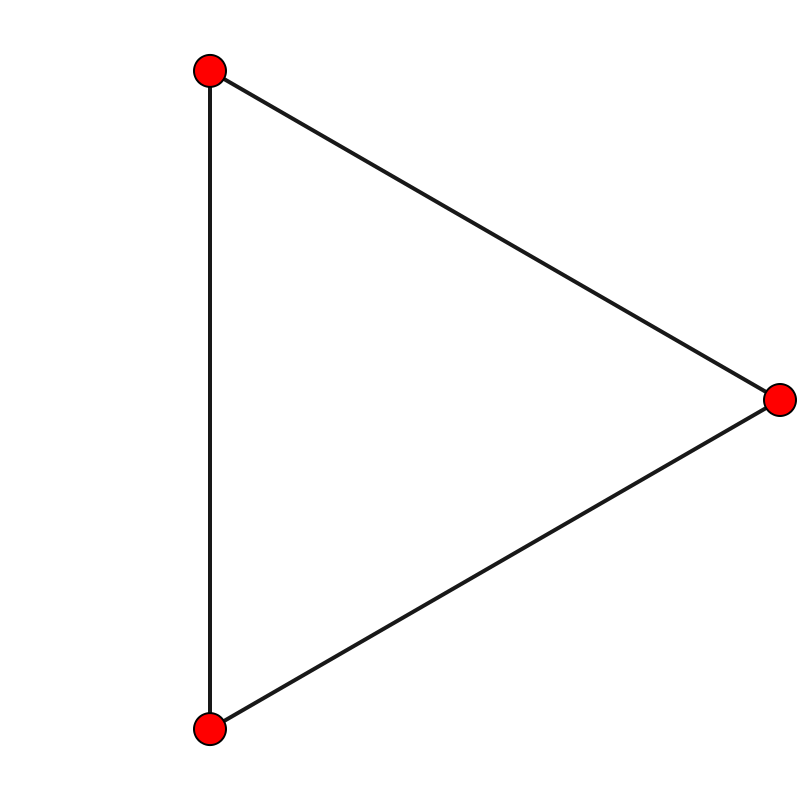
\includegraphics[width=0.4\textwidth]{img/800px-2-simplex_t0.png}
    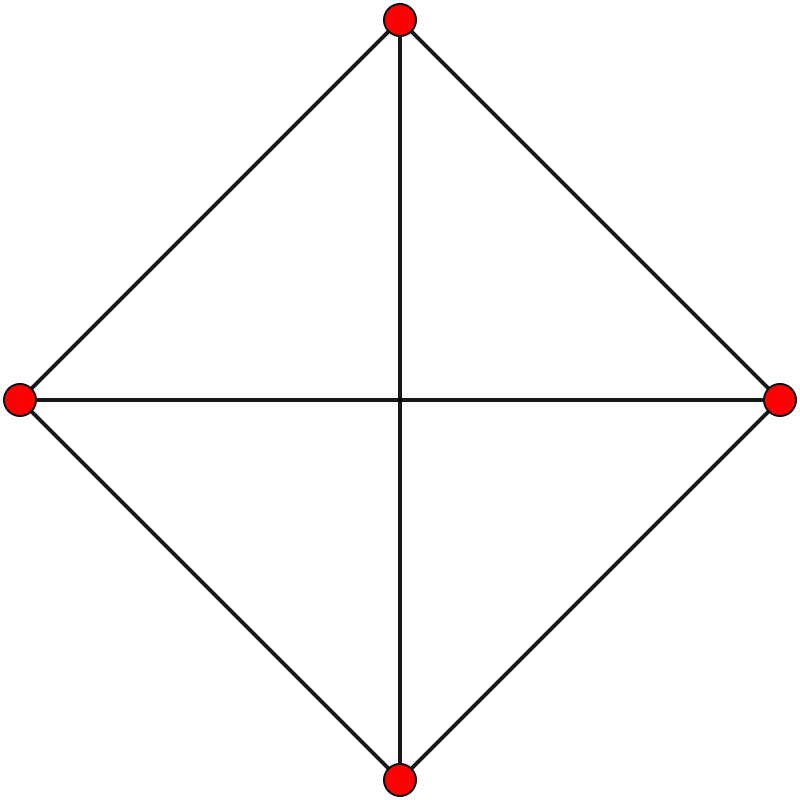
\includegraphics[width=0.4\textwidth]{img/800px-3-simplex_t0.png}
    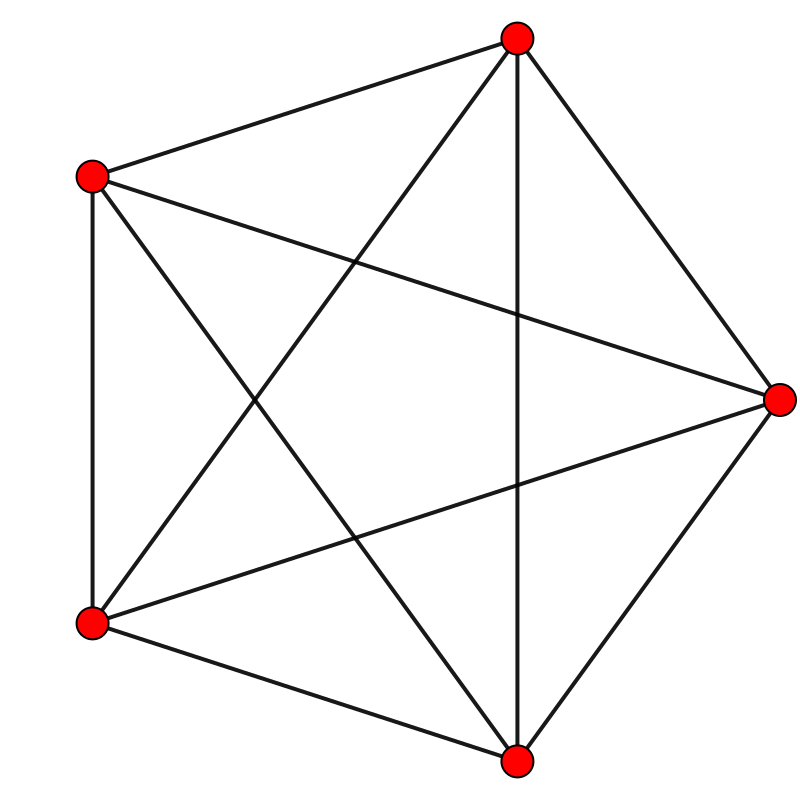
\includegraphics[width=0.4\textwidth]{img/800px-4-simplex_t0.png}
  \caption{Examples of Simplices}
  \label{fig:simplices}
\end{figure}

We notice that the 1-simplex is formed by two 0-simplices, a 2-simplex is formed
by three 1-simplices, and the 3-simplex by four 2-simplices. The components of
these compositions are called ``faces", in a similar manner to the polyhedra. The 0-face is often called a vertex
and the 1-face an edge. If we tabled the quantities of each M-face in an
N-simplex out, they form
Pascal's triangle and thus follow the binomial coefficient.

\begin{equation}
{N+1}\choose{M+1}
\end{equation}

Simplices will be our most basic geometry we use for formulating the combinatorial
form of a polytope. In fact, the two- and three-simplices are already
polytopes and adhere to Coxeter's definition! To generalize independent of
a vector, we will define a self-referential abstract form. In order to
accomplish this we will introduce a notation of a simplex using a syntax
that will be expanded in the computation section. We will let the order
or dimensionality, $N$ of
a simplex be denoted by $Simplex\{N\}$, where the brackets are the parameter
for the dimensionality. Given points $P$, let $Simplex\{0\}(P_1) = P_1$.
Then $Simplex\{1\}(Simplex\{0\}(P_1), Simplex\{0\}(P_2))$ is the construction
of a one-simplex. If we have our assumption for the 0-simplex we may
abstractly define the construction of a simplex of order N without convex
hulls by a recursive relation. A $Simplex\{N\}$ is constructed by
$Simplex\{N-1\}$ in the quantity ${N+1}\choose{N}$.
Such a construction terminates since
a $Simplex\{0\}$ is a point. However for most practical purposes
we may simply specify an N-simplex as a set of $N+1$ points.

\todo{P is a set of vectors}

\subsubsection{Orientation}

Before we proceed to construct a polytope with simplices we will
discuss orientation on a simplex. The orientation of a simplex is the
direction an edge assumes from the ordering. This is simplest to
explain in terms of the 

\begin{figure}[h!]
  \centering
    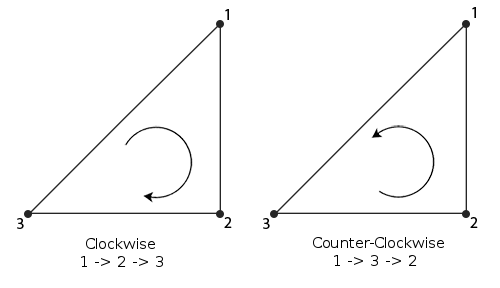
\includegraphics[width=0.75\textwidth]{img/Winding_order.png}
  \caption{The two possible orientations of a triangle given 3 points.}
  \label{fig:tri_orientation}
\end{figure}



%\todo{John M. Lee Introduction to Topological Manifolds}
%\cite{Lee_2011}

%We now have the tools neccesary to construct a combinatorial representation
%of a polytope. In the functional representation we were interested in
%extracting geometric information about points and their distances from the
%polytope. The combinatorial representation will help us observe the
%relationships between the faces. To construct an N-polytope we will use 
%N-1 simplices. using set 

%\subsection{Construction of the Combinatorial Representation}

%In our previous discussion of simplices we have roughly explained
%the recursive nature. 

%\section{Implicit Functional Representations of Solids}

%\subsection{Hyperplanes}

%In multiple dimensions this is more interesting since we may construct
%various, rather arbitrary, geometries to make a closed space.
%One common example is a hyperplane. A hyperplane is simply a generalization
%of the a plane into arbitrary dimensions, with the property it is
%of dimensionality N-1. For example if we are in 2D space, our hyperplane
%is a line since it partitions our space into two parts. Likewise in 3D
%space this is a plane. If we define a hyperplane functionally using vector
%notation we can extract some interesting properties.
%For simplicity in this example let us assume we have a hyperplane which
%cuts through the origin.
%If we let 
%$\vec{x}$ be an arbitrary point in $N$ dimensional space,
%and $\vec{a}$ be the slopes of each axis, then one functional construction is
%simply the dot product, $dot(\vec{a},\vec{x})$. If x is on the hyperplane
%the function will be equal to zero. If it is not zero,
%then we may determine which side of the partition the point lies on.
%Thus as a set representation the hyperplane is:

%\begin{equation}
%\{f(x)=dot(\vec{a},\vec{x})|f(x)=0,x \in \mathbb{R}\}
%\end{equation}

%\todo{define hyperplane sooner}
%We notice that the hyperplane cuts space, but does not create a closed
%subspace. What we are after is a "solid", which is the composition of
%such objects forming a closed space. In fact, this leads to a proper definition
%of a closed set in topology. We will say that \emph{a set is closed if and only if it
%contains all of its limits}\cite{007054235X}. In the case of the lone hyperplane
%it is not bounded, so itself therefore not closed (by not having limits). Thus
%we must compose hyperplanes to form closed spaces!


%\todo{Implicit Surface and Distance Field}

%If we were to functionally define the boundary of a solid a predicate of the
%form $f(x) = 0$ would suffice, where the solid is defined by all $x$.
%However we previously mentioned that it is
%useful in computation to define a function that returns infomation about
%the membership of a point in the solid. Further more we can define our functional
%solid to return a value corresponding to the shortest distance to the boundary.\cite{Olah_2011}
%These functions are sometimes called "implicit" forms in solid modelling, but
%more precisely they generate a distance field.

%A sketch of this behavior in one dimension
%can be seen in Figure \ref{fig:implicit-sketch}.

%\begin{figure}[h!]
%  \centering
%    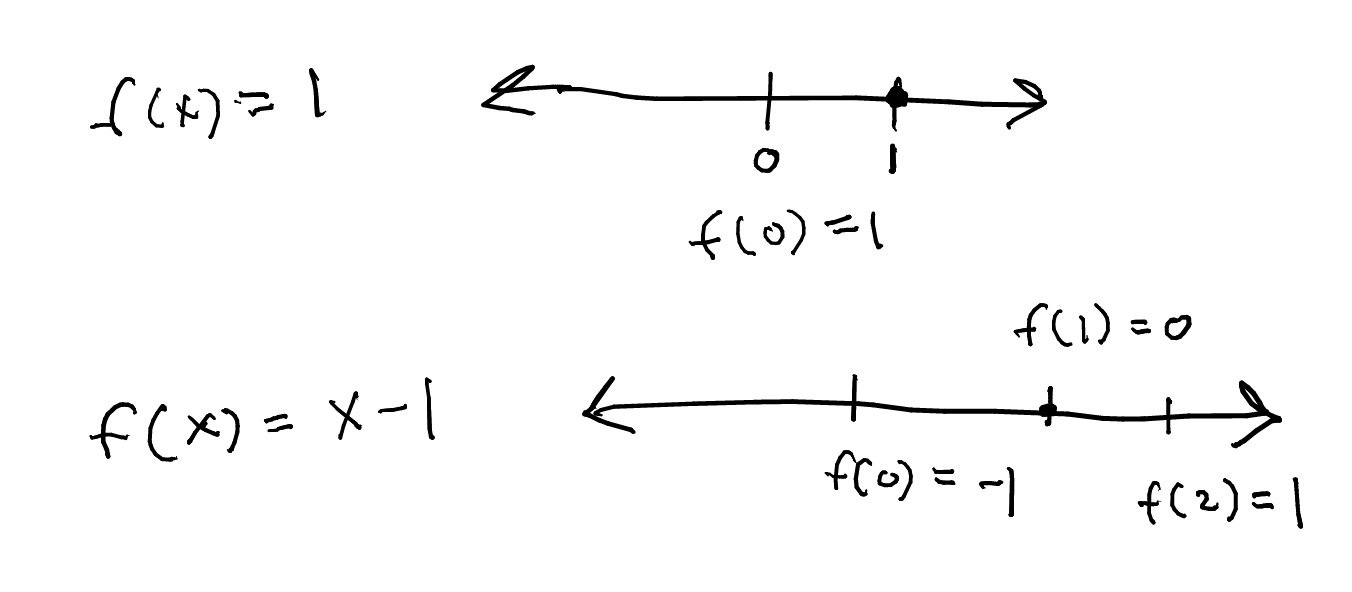
\includegraphics[width=0.75\textwidth]{img/implicit_sketch.png}
%  \caption{Number line illustrating the construction of an implicit signed function}
%  \label{fig:implicit-sketch}
%\end{figure}

%\subsubsection{Affine Transforms}

%Functional representations can naturally deal with affine
%transforms\cite{Henderson_2002}. Given some transform associated with a
%solid, one simply applies the inverse transform to check membership.
%The key word here is "associated" since for our purposes we will define
%geometries without consideration of their tranforms. This is one aspect
%in which computation will aid us extensively. If we let $f$ be a functional
%representation of a solid or spatial partition
%which generates a signed distance field, $A$ be the transform of the object,
%and $x$ be the point whose membership in the solid is in question. It then
%follows that the distance field formed by $f$ transformed by $A$ is obtained
%by $f(A^{-1}*x)$.

%\begin{figure}[h!]
%  \centering
%    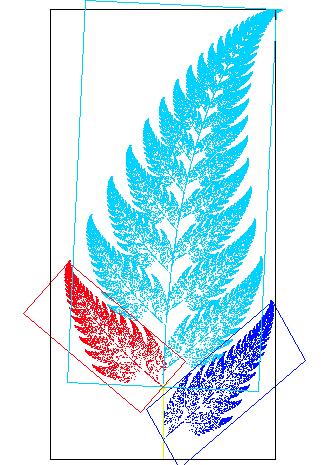
\includegraphics[width=0.5\textwidth]{img/Fractal_fern_explained.png}
%  \caption{Number line illustrating the construction of an implicit signed function}
%  \label{fig:implicit-sketch}
%\end{figure}

%\todo{Affines are groups}

%\subsubsection{Orientation}


%\subsection{Set operations on Distance Fields}


%One can also compose distance fields with logical operations. 
%Below are basic set operations defined for these functions using our
%sign conventions:

%\begin{equation*}
%\cap : \mathtt{min}(f_1,f_2) \\
%\end{equation*}
%\begin{equation*}
%\cup : \mathtt{max}(f_1,f_2) \\
%\end{equation*}
%\begin{equation*}
%\neg : -\mathtt{f}_1
%\end{equation*}

%\todo{proof/cite}

%It follows that the ``difference"
%of $f_1$ and $f_2$ is the intersection of $f_1$ with the negation of $f_2$,
%$\mathtt{max}(f_1,-f_2)$. Thus we may compose functional representations
%of geometry using the language of set operations, namely, union, difference,
%intersection, and negation.
%The mathematical analyst might have trouble with these formulations because
%such operations create discontinuities. To illucidate this problem we may
%use the language of norms. A distance field as we have defined it behaves
%like the inf-norm, or maximum norm. If we choose a point and take a projection
%to the surface which forms the shortest path, our distance value
%will be linear. This is not very useful for any kind of differential
%analysis since we only have first order derivatives.
%It may be useful for a parametric mathematical construction of a polytope
%to have differentiable properties. Rvachev functions
%provide one solution to this problem.


%\subsubsection{Rvachev Functions}

%In the 1960's Vladimir Rvachev produced a method for handling the "inverse
%problem of analytic geometry". His theory consists of functions which provide a
%link between logical and set operations in geometric modeling and analytic
%geometry.\cite{shapiro1991theory} While attempting to solve boundary value problems,
%Rvachev formulated an equation of a square as
%\begin{equation*}
%a^2 + b^2 − x^2 − y^2 + \sqrt[]{( a^2 − x^2 )^2 +( b^2 − y^2 )^2} =0
%\end{equation*}

%Implicitly, the sides of a square can be defined as $x= +/- a$ and $y= +/- b$.
%The union of these two is a square. By reducing the formulation of the square
%he generalized an expression for the union between two functions.
%\begin{equation*}
%\cup : f_1 + f_2 + \sqrt[]{f_1^2 +f_2^2} = 0
%\end{equation*}

%Likewise we can see that intersections and negations can be formed for logical
%completion.
%\begin{equation*}
%\cap : f_1 + f_2 - \sqrt[]{f_1^2 +f_2^2} =0 \\
%\end{equation*}
%\begin{equation*}
%\neg : -f_1
%\end{equation*}

%These formulations can be modified for $C^m$ continuity for any $m$.

%\todo{clean}

%The Rvachev construction is of hypothetical interest in the presentation,
%but shows how geometric
%constructions can converge with analytic constructions.

%In 2000 Rvachev published an english-language proof of the completeness
%\cite{Rvachev_Sheiko_Shapiro_Tsukanov_2000}

%\cite{shapiro2007semi} In addition Pasko, et. al. have shown that Rvachev
%functions can serve to replace a geometry kernel by creating logical
%predicates. \cite{pasko1995function} Their research also establishes the
%grounds for user interfaces and environment description. For this work a
%practical implementation will most likely leverage their insights.
%Rvachev and Shapiro have also shown that using the POLE-PLAST and SAGE
%systems a user can generate complex semi-analytic geometry
%as well.\cite{rvachev2000completeness} 

%One of the most general expositions in the English language of R-Functions
%applied to BVPs is
%Vadim Shapiro's``Semi-Analytic Geometry with R-Functions". \cite{shapiro2007semi}
%Unfortunately, no monographs about R-Functions exist in the English literature.
%Most literature is in Russian, however many articles presenting applied
%problems using the R-Function Method. \cite{voron2010}

%Such a system for analytic geometry can be developed further. In the context
%of an Eulerian flow field, a distance field over a function that
%generates partial derivatives could be a fast numerical computation method.

%\todo{clean}



%\subsection{Construction of the Implicit Functional Representation}

%We now have the mathematical concepts needed to define a polytope using the
%language of hyperplanes. Using vector notation we may define a hyperplane 
%as an implicit function generating a distance field by:

%\begin{equation}
%f(x) = \frac{a \cdot x }{\sqrt{a \cdot a}}
%\end{equation}

%where $a$ are the slopes and $x$ being the point in question. This function
%will be zero when $x$ lies on the plane.

%\cite{Polyhedra}

%\section{Spacial Terminology}


%\subsection{Solids}

%Before we define a polyhedra, we must introduce a few notions. These are
%solids and orientation. Solids have been studied since
%antiquity and for our purposes we will define them as constructions in
%three dimensional space with finite volume.
%For example, a plane which partitions space is not a solid
%since either partition is unbounded, however the intersection of planes
%could form a solid.

%Orientation is a parallel concept which allows us to specify how geometric
%objects contain space. As an example, let us go back to our partition of
%space with a plane. If we are on our way to construct a solid, it is
%neccessary to choose the one part to keep and the other to discard. This is
%the purpose of orientation. In the case of the plane, this follows from the
%definition, $ax+by+cz+d=0$. More lucidly, lets look at the signed distance
%of a point from the plane, computed as:
%\begin{equation}
%D = \frac{ax+by+cz+d}{\sqrt{a^2+b^2+c^2}}
%\end{equation}
%For simplicity, let's look at a plane parallel to the X and Y axes passing
%through z = 1. Thus $a$ and $b$ are set to 0, $c$ set to 1, and
%$d=-1$
%Simplifying our formulation we have:
%\begin{equation}
%D = 0x+0y+z-1 = z-1
%\end{equation}
%At $z=1$ we see we are on the plane, however at $z=0$ and $z=2$ we get -1 and 1
%respectively. The sign of the distance is our indicator of orientation. We can
%choose an arbitrary convention as to which partition we will count, but akin
%to the "right hand rule" in physics, the normals of the partition must point
%outwards. In the case of the plane the normal is the vector $(a,b,c)$, which
%in our realization is the upwards vector $(0,0,1)$. Since the convention is
%such that the normals point outward, the partition we would consider in a
%solid is all points \emph{in the opposite direction of the normal}.
%Also to note is the importance of sign in our distance function. We can exploit
%this behavior to indicate containment when performing set operations on
%spatial partitions. Negative values thus indicate a point inside the partition
%of interest. We have chosen this convention for this paper due to
%it's ubiquity in computation frameworks. In the field of computer graphics
%using descrete polytopes, this is often referred to as "winding order".


